\documentclass[25pt,a0paper,landscape]{tikzposter}
\usetheme{Board}
\usepackage[utf8]{inputenc}
\usepackage{xurl}
\usepackage{natbib}
\usepackage{amsmath,amssymb}
\usepackage{pstricks}
\usepackage{pst-barcode}
% \usepackage{iftex}
\usepackage{textcomp} % provide euro and other symbols
% \usepackage{lmodern}
% % Use upquote if available, for straight quotes in verbatim environments
% \IfFileExists{upquote.sty}{\usepackage{upquote}}{}
% \IfFileExists{microtype.sty}{% use microtype if available
%   \usepackage[]{microtype}
%   \UseMicrotypeSet[protrusion]{basicmath} % disable protrusion for tt fonts
% }{}
% \makeatletter
% \@ifundefined{KOMAClassName}{% if non-KOMA class
%   \IfFileExists{parskip.sty}{%
%     \usepackage{parskip}
%   }{% else
%     \setlength{\parindent}{0pt}
%     \setlength{\parskip}{6pt plus 2pt minus 1pt}}
% }{% if KOMA class
%   \KOMAoptions{parskip=half}}
% \makeatother
\usepackage{xcolor}
% Define solarized colors
\definecolor{solarized-base03}{HTML}{002b36}
\definecolor{solarized-base02}{HTML}{073642}
\definecolor{solarized-base01}{HTML}{586e75}
\definecolor{solarized-base00}{HTML}{657b83}
\definecolor{solarized-base1}{HTML}{839496}
\definecolor{solarized-base2}{HTML}{93a1a1}
\definecolor{solarized-base3}{HTML}{e7e9db}
\definecolor{solarized-yellow}{HTML}{b58900}
\definecolor{solarized-orange}{HTML}{cb4b16}
\definecolor{solarized-red}{HTML}{dc322f}
\definecolor{solarized-magenta}{HTML}{d33682}
\definecolor{solarized-violet}{HTML}{6c71c4}
\definecolor{solarized-blue}{HTML}{268bd2}
\definecolor{solarized-cyan}{HTML}{2aa198}
\definecolor{solarized-green}{HTML}{859900}

\setlength{\emergencystretch}{3em} % prevent overfull lines
\providecommand{\tightlist}{%
  \setlength{\itemsep}{0pt}\setlength{\parskip}{0pt}}
\setcounter{secnumdepth}{-\maxdimen} % remove section numbering
\usepackage{tikz}
\usepackage{tikz-cd}
\usepackage[most]{tcolorbox}
\usetikzlibrary{decorations.pathmorphing,shadows.blur,shadings}
\tcbuselibrary{skins}
%\pgfmathsetseed{1} % To have predictable results

% Define a background layer, in which the parchment shape is drawn
% \pgfdeclarelayer{background}
% \pgfsetlayers{background,main}

% This is the base for the fractal decoration. It takes a random point
% between the start and end, and raises it a random amount, thus
% transforming a segment into two, connected at that raised point This
% decoration can be applied again to each one of the resulting
% segments and so on, in a similar way of a Koch snowflake.
\pgfdeclaredecoration{irregular fractal line}{init}
{
  \state{init}[width=\pgfdecoratedinputsegmentremainingdistance]
  {
    \pgfpathlineto{%
      \pgfpoint{random * \pgfdecoratedinputsegmentremainingdistance}{%
        (random * \pgfdecorationsegmentamplitude - 0.02) *
         \pgfdecoratedinputsegmentremainingdistance}}
    \pgfpathlineto{\pgfpoint{\pgfdecoratedinputsegmentremainingdistance}{0pt}}
  }
}

% Define paper style
\tikzset{
  paper/.style={%
    draw=black!10,
    blur shadow,
    path picture={%
      \fill[solarized-base3!50!white] ([shift={(-5pt,-5pt)}]path picture bounding box.south west) rectangle ([shift={(5pt,5pt)}]path picture bounding box.north east);
    }
  },
  irregular border/.style={%
    decoration={irregular fractal line, amplitude=0.2},
    decorate,
  },
  ragged border/.style={%
    decoration={random steps, segment length=7mm, amplitude=2mm},
    decorate,
  }
}

\newtcolorbox{quotebox}{%
  % enhanced jigsaw, <-- Beware, This rendering engine let the
  %                      frame appear on some PDF viewers
  empty, % Better use this rendering engine to avoid the bug
  interior code={%
    % \begin{pgfonlayer}{background}  % Draw the shape behind
      \fill[paper] % recursively decorate the bottom border
      decorate[irregular border]{%
        decorate{decorate{decorate{decorate[ragged border]{
                ($(interior.south east) - (0, random * 5mm)$) --
                ($(interior.south west) - (0, random * 5mm)$)
              }
            }
          }
        }
      }
      -- (interior.north west) -- (interior.north east) -- cycle;
    % \end{pgfonlayer}
  },
  sharp corners,
  boxrule=0pt,
  left=5pt,
  right=5pt,
  top=5pt,
  bottom=0.5em,
  after skip=10mm,
}

%% TColorBox Note environment
\newlength\savedparindent
\setlength\savedparindent\parindent
\newenvironment{tnote}[1]{%
  \begin{tcbnote}{}
    \setlength\parindent{\savedparindent}
    \begin{center}
      \sffamily\bfseries\LARGE #1
    \end{center}\par
  }{%
  \end{tcbnote}
}
% Color box styles
\newtcolorbox{tldrbox}{
  colback=solarized-blue!5!white,
  colframe=solarized-blue!75!black,
  title=TL;DR,
  enhanced,
  drop shadow southeast,
  boxrule=2pt,
  fonttitle=\bfseries\large,
  sharp corners=south,
  rounded corners=north,
  interior style={top color=solarized-blue!5!white, bottom color=solarized-blue!20!white}, 
}
\newtcolorbox{proofbox}[1][]{
  colback=solarized-cyan!5!white,
  colframe=solarized-cyan!75!black,
  enhanced,
  drop shadow southeast,
  boxrule=2pt,
  sharp corners=south,
  rounded corners=north,
  interior style={top color=solarized-cyan!1!white, bottom color=cyan!5!white}, 
  #1
}
\newtcolorbox{theorybox}[1][]{
  colback=solarized-yellow!5!white,
  colframe=solarized-yellow!75!black,
  enhanced,
  drop shadow southeast,
  boxrule=2pt,
  sharp corners=south,
  rounded corners=north,
  interior style={top color=solarized-yellow!5!white, bottom color=solarized-yellow!10!white}, 
  #1
}
\newtcolorbox{examplebox}[1][]{
  colback=solarized-violet!5!white,
  colframe=solarized-violet!75!black,
  enhanced,
  drop shadow southeast,
  boxrule=2pt,
  sharp corners=south,
  rounded corners=north,
  interior style={top color=solarized-violet!5!white, bottom color=solarized-violet!10!white}, 
  #1
}
\newtcolorbox{backgroundbox}[1][]{
  colback=solarized-base00!5!white,
  colframe=solarized-base00!75!black,
  enhanced,
  drop shadow southeast,
  boxrule=2pt,
  sharp corners=south,
  rounded corners=north,
  interior style={top color=solarized-base00!5!white, bottom color=solarized-base00!10!white}, 
  #1
}


\usepackage{graphicx}
\usepackage{multicol}
\usepackage{amsmath,amsfonts,amssymb,amsthm,bm}
\usepackage{mathtools}
\DeclareMathOperator{\opExpectation}{\mathbb{E}}
\newcommand{\E}[2]{\opExpectation_{#1} \left [ #2 \right ]}
\newcommand{\simpleE}[1]{\opExpectation_{#1}}
\newcommand{\MidSymbol}[1][]{\:#1\:}
\newcommand{\given}{\MidSymbol[\vert]}
\DeclareMathOperator{\opmus}{\mu^*}
\newcommand{\IMof}[1]{\opmus[#1]}
\DeclareMathOperator{\opInformationContent}{H}
\newcommand{\ICof}[1]{\opInformationContent[#1]}
\newcommand{\xICof}[1]{\opInformationContent(#1)}
\DeclareMathOperator{\opEntropy}{H}
\newcommand{\Hof}[1]{\opEntropy[#1]}
\newcommand{\xHof}[1]{\opEntropy(#1)}

\DeclareMathOperator{\opMI}{I}
\newcommand{\MIof}[1]{\opMI[#1]}
\DeclareMathOperator{\opTC}{TC}
\newcommand{\TCof}[1]{\opTC[#1]}
\newcommand{\CrossEntropy}[2]{\opEntropy(#1 \MidSymbol[\Vert] #2)}
\DeclareMathOperator{\opKale}{D_\mathrm{KL}}
\newcommand{\Kale}[2]{\opKale(#1 \MidSymbol[\Vert] #2)}
\DeclareMathOperator{\opJSD}{D_\mathrm{JSD}}
\newcommand{\JSD}[2]{\opJSD(#1 \MidSymbol[\Vert] #2)}
\newcommand{\opp}{\mathrm{p}}
\newcommand{\pof}[1]{\opp(#1)}
\newcommand{\hpof}[1]{\hat{\opp}(#1)}
\newcommand{\pcof}[2]{\opp_{#1}(#2)}
\newcommand{\hpcof}[2]{\hat\opp_{#1}(#2)}
\newcommand{\opq}{\mathrm{q}}
\newcommand{\qof}[1]{\opq(#1)}
\newcommand{\hqof}[1]{\hat{\opq}(#1)}
\newcommand{\qcof}[2]{\opq_{#1}(#2)}
\newcommand{\varHof}[2]{\opEntropy_{#1}[#2]}
\newcommand{\xvarHof}[2]{\opEntropy_{#1}(#2)}
\newcommand{\varMIof}[2]{\opMI_{#1}[#2]}
\newcommand{\w}{\boldsymbol{\theta}}
\newcommand{\W}{\boldsymbol{\Theta}}
\newcommand{\opf}{\mathrm{f}}
\newcommand{\fof}[1]{\opf(#1)}
\newcommand{\Dany}{\mathcal{D}}
\newcommand{\y}{y}
\newcommand{\Y}{Y}
\newcommand{\Loss}{\boldsymbol{L}}
\newcommand{\x}{\boldsymbol{x}}
\newcommand{\X}{\boldsymbol{X}}
\newcommand{\pdata}[1]{\hpcof{\text{data}}{#1}}
\newcommand{\normaldist}[1]{\mathcal{N}(#1)}
\urlstyle{same}
% \hypersetup{
%   pdftitle={Bridging the Data Processing Inequality and Function-Space Variational Inference},
%   pdfauthor={Andreas Kirsch, University of Oxford},
%   hidelinks}

\renewcommand{\bibsection}{} % This line disables the automatic "References" section heading

\title{Data Processing Inequality \raisebox{0em}{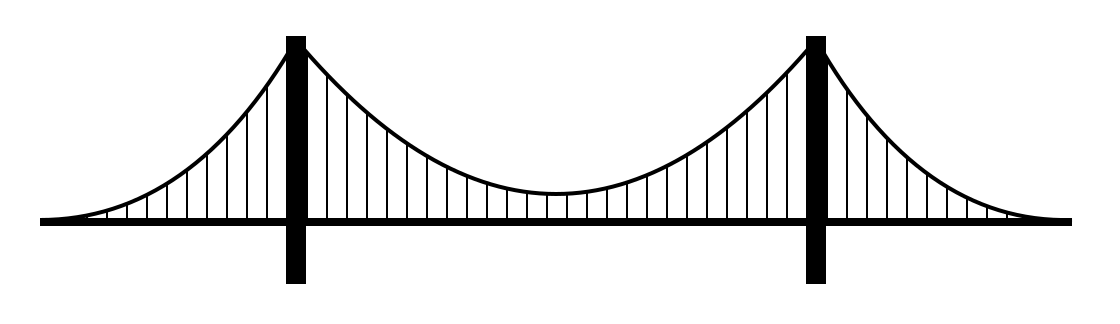
\includegraphics[height=1em]{Suspension_bridge_icon.svg.png}} Function-Space Variational Inference}
\author{Andreas Kirsch}
\institute{University of Oxford\textsuperscript{--2023}}
\date{\today}

\begin{document}
\maketitle

\begin{columns}
  \column{0.5}
  \block{Data Processing Inequalities}{
  \begin{tldrbox}
    Informally, the \textbf{Data Processing Inequality (DPI)} states that processing data stochastically can only reduce information. 
    Formally, for distributions $\mathrm{q}(\boldsymbol{\Theta})$ and $\mathrm{p}(\boldsymbol{\Theta})$ over a random variable $\boldsymbol{\Theta}$ and a stochastic mapping $Y = \mathrm{f}(\boldsymbol{\Theta})$, the Kullback-Leibler DPI is expressed as:
    $$\mathop{\mathrm{D_\mathrm{KL}}}(\mathrm{q}(\boldsymbol{\Theta}) \:\Vert\: \mathrm{p}(\boldsymbol{\Theta})) \ge \mathop{\mathrm{D_\mathrm{KL}}}(\mathrm{q}(Y) \:\Vert\: \mathrm{p}(Y))$$
    Equality holds when $\mathop{\mathrm{D_\mathrm{KL}}}(\mathrm{q}(\boldsymbol{\Theta}\:\vert\:Y) \:\Vert\: \mathrm{p}(\boldsymbol{\Theta}\:\vert\:Y)) = 0$.
  \end{tldrbox}
  \begin{multicols}{2}
  \begin{quotebox}
    {\Large\emph{The data processing inequality states that if two random variables are transformed in this way, they cannot become easier to tell apart.}}
    \begin{flushright}
    ``Understanding Variational Inference in Function-Space'', \\
    Burt et al. (2021)
    \end{flushright}
  \end{quotebox}
  \begin{examplebox}[title=Example: Image Processing]
    Consider an image processing pipeline where $X$ is the original image, $Y$ is a compressed version, and $Z$ is $Y$ after adding blur and pixelation. The DPI tells us that the mutual information $\mathop{\mathrm{I}}[X;Y] \ge \mathop{\mathrm{I}}[X;Z]$, as each processing step results in information loss.
  \end{examplebox}
\end{multicols}
\begin{multicols}{2}
  \begin{theorybox}[title=Jenson-Shannon Divergence DPI]
  The Jensen-Shannon divergence (JSD) makes the KL divergence symmetric. For:
  \begin{align*}
  \mathrm{f}(x) &= \frac{\mathrm{p}(x) + \mathrm{q}(x)}{2}\\
  \mathop{\mathrm{D_\mathrm{JSD}}}(\mathrm{p}(x) \:\Vert\: \mathrm{q}(x)) &= \frac{1}{2} \mathop{\mathrm{D_\mathrm{KL}}}(\mathrm{p}(x) \:\Vert\: \mathrm{f}(x)) + \frac{1}{2} \mathop{\mathrm{D_\mathrm{KL}}}(\mathrm{q}(x) \:\Vert\: \mathrm{f}(x)).
  \end{align*}
  The square root of the Jensen-Shannon divergence, the \emph{Jensen-Shannon distance}, is symmetric, satisfies the triangle inequality, and is hence a metric.

  For $\mathrm{p}(x)$ and $\mathrm{q}(x)$ and a shared transition function $\mathrm{f}(y \:\vert\:x)$ for the model $X \rightarrow Y$, we apply the KL DPI twice and obtain the JSD DPI:
  %, we obtain a Jensen-Shannon divergence data processing inequality by applying the KL DPI twice:
  $$
  \mathop{\mathrm{D_\mathrm{JSD}}}(\mathrm{p}(X) \:\Vert\: \mathrm{q}(X)) \ge \mathop{\mathrm{D_\mathrm{JSD}}}(\mathrm{p}(Y) \:\Vert\: \mathrm{q}(Y)).
  $$
  \end{theorybox}
  \begin{theorybox}[title=Mutual Information DPI]  
  For any Markov chain $Z \rightarrow X \rightarrow Y$ with $\mathrm{f}(z, x, y) = \mathrm{f}(z) \mathrm{f}(x \:\vert\:z) \mathrm{f}(y \:\vert\:x)$ for any distribution $\mathrm{f}(z)$, we have:
  \begin{align*}
    \MIof{X;Z} &= \Kale{\fof{X \given Z}}{\fof{X}}\\
    &= \E{\fof{z}} {\Kale{\fof{X \given z}}{\fof{X}}}\\
    &\overset{(1)}{\ge} \E{\fof{z}} {\Kale{\fof{Y \given z}}{\fof{Y}}}\\
    &= \Kale{\fof{Y \given Z}}{\fof{Y}}\\
    &= \MIof{Y;Z},
  \end{align*}
  where $(1)$ follows from the KL DPI.
  %This is the data processing inequality for the mutual information.
  \end{theorybox}
% \end{multicols}
% }
% \block{Proofs}{
%   \begin{multicols}{2}
  \begin{backgroundbox}[title={Chain Rule of the 
\includegraphics[width=1em]{leafy-green.png} Divergence}]
    An important property of the KL divergence is the chain rule:
    \begin{align*}
    &\Kale{\qof{\Y_n,...}}{\pof{\Y_n,...}} \\
    &\quad = \sum_{i=1}^n \Kale{\qof{\Y_i \given 
    \Y_{i-1}, ...}}{\pof{\Y_i \given \Y_{i-1}, ...}}.
    \end{align*}
  \end{backgroundbox}
  \begin{proofbox}[title={Proof of the 
\includegraphics[width=1em]{leafy-green.png} DPI}]
    Using the chain rule of the KL divergence twice:
    % \begin{align*}
    % \mathop{\mathrm{D_\mathrm{KL}}}(\mathrm{p}(X, Y) \:\Vert\: \mathrm{q}(X, Y)) &= \mathop{\mathrm{D_\mathrm{KL}}}(\mathrm{p}(X) \:\Vert\: \mathrm{q}(X)) \\
    % &+ \mathop{\mathrm{D_\mathrm{KL}}}(\mathrm{p}(Y \:\vert\:X) \:\Vert\: \mathrm{q}(Y \:\vert\:X)),
    % \end{align*}
    % and its symmetry, we have:
    \begin{align*}
    &\mathop{\mathrm{D_\mathrm{KL}}}(\mathrm{p}(X) \:\Vert\: \mathrm{q}(X)) + \underbrace{\mathop{\mathrm{D_\mathrm{KL}}}(\mathrm{p}(Y\:\vert\:X) \:\Vert\: \mathrm{q}(Y \:\vert\:X))}_{=\mathop{\mathrm{D_\mathrm{KL}}}(\mathrm{f}(Y\:\vert\:X) \:\Vert\: \mathrm{f}(Y \:\vert\:X))=0}\\
    &\quad =\mathop{\mathrm{D_\mathrm{KL}}}(\mathrm{p}(X, Y) \:\Vert\: \mathrm{q}(X, Y))\\
    &\quad =\mathop{\mathrm{D_\mathrm{KL}}}(\mathrm{p}(Y) \:\Vert\: \mathrm{q}(Y))+\underbrace{\mathop{\mathrm{D_\mathrm{KL}}}(\mathrm{p}(X \:\vert\:Y) \:\Vert\: \mathrm{q}(X \:\vert\:Y))}_{\ge 0}\\
    &\quad \ge \mathop{\mathrm{D_\mathrm{KL}}}(\mathrm{p}(Y) \:\Vert\: \mathrm{q}(Y)).
    \end{align*}
    We have equality exactly when $\mathrm{p}(x \:\vert\:y) = \mathrm{q}(x \:\vert\:y)$ for (almost) all $x, y.$
  \end{proofbox}
  \begin{theorybox}[title={Chain Rule of the 
\includegraphics[width=1em]{leafy-green.png} DPI}]
    The DPI also yields a \textbf{chain inequality}:
    \begin{align*}
    \Kale{\qof{\Y_n,...}}{\pof{\Y_n,...}} &\ge \Kale{\qof{\Y_{n-1},...}}{\pof{\Y_{n-1},...}} \\
    &...\\
    &\ge \Kale{\qof{\Y_1}}{\pof{\Y_1}},
    \end{align*}
    where we start from the KL DPI and then use the chain rule. 
  \end{theorybox}
  \end{multicols}
}
% \column{0.25}
% \block{Variational Inference \& ELBO}{
%   In standard VI, we approximate a Bayesian posterior $\pof{\w \given \Dany}$ with a variational distribution $\qof{\w}$ by minimizing $\Kale{\qof{\W}}{\pof{\W \given \Dany}}$.
%     This yields an information-theoretic evidence (\textbf{upper}) bound on the information content $-\log \pof{\Dany}$ of the data $\Dany$ under the variational distribution $\qof{\w}$:
%     \begin{align*}
%     & \underbrace{-\log \pof{\Dany}}_{\text{Evidence }\xHof{\pof{\Dany}}} \le \xHof{\pof{\Dany}} + \Kale{\qof{\W}}{\pof{\W \given \Dany}} \\
%     &= \xHof{\pof{\Dany}} + \Kale{\qof{\W}}{\frac{\pof{\Dany \given \W}\,\pof{\W}}{\pof{\Dany}}}\\
%     &\, = \underbrace{\E{\qof{\w}}{-\log \pof{\Dany \given \w}} + \Kale{\qof{\W}}{\pof{\W}}}_{\text{Evidence}\ \text{Bound}}.
%     \end{align*}
%     In the literature, the negative of this bound is called the \textbf{evidence lower bound (ELBO)} and is maximized.
% }
\begin{subcolumns}
  \subcolumn{0.25}
  \block{Full Blog Post}{
    % \begin{tikzpicture}
      \centering
      
\includegraphics[width=0.0625\textwidth]{fsvi_qr_code.png}
    % \end{tikzpicture}
  }
  \subcolumn{0.75}
  \block{More References}{
    % Add references from assets/bibliography/2024-05-07-dpi-fsvi.bib
    \nocite{cover1999elements,rudner2022tractable}
    \bibliographystyle{plain}
    \bibliography{fsvi_poster}
  }
\end{subcolumns}
\column{0.5}
\block{Function-Space Variational Inference}
{
  \begin{tldrbox}
    \textbf{Function-space variational inference (FSVI)} is a principled approach to Bayesian inference that respects the inherent symmetries and equivalences in overparameterized models. It focuses on approximating the meaningful posterior $\pof{[\w] \given \Dany}$ over prediction equivalence classes of the parameters while avoiding the complexities of explicitly constructing and working with equivalence classes.
    The FSVI-ELBO regularizes towards a data prior using the KL DPI:
    \begin{align*}
    \E{\qof{\w}}{-\log \pof{\Dany \given \w}} + \Kale{\qof{\Y... \given \x...}}{\pof{\Y... \given \x...}},
    \end{align*}
    (unlike in regular variational inference, where we regularize towards a parameter prior $\Kale{\qof{\W}}{\pof{\W}}$).
  \end{tldrbox}
  \begin{multicols}{2}
    \begin{backgroundbox}[title=(Regular) Variational Inference \& ELBO]
      The Bayesian posterior $\pof{\w \given \Dany}$ is approximated with a variational distribution $\qof{\w}$ by minimizing $\Kale{\qof{\W}}{\pof{\W \given \Dany}}$. Dropping constant (intractable) terms yields a simplified tractable objective, which \textbf{upper} bounds the information content $-\log \pof{\Dany}$ of the data $\Dany$:
      \begin{align*}
      & 0 \le \Kale{\qof{\W}}{\pof{\W \given \Dany}} \\
      &= \Kale{\qof{\W}}{\frac{\pof{\Dany \given \W}\,\pof{\W}}{\pof{\Dany}}}\\
      &\, = \underbrace{\E{\opq}{-\log \pof{\Dany \given \W}} + \Kale{\qof{\W}}{\pof{\W}}}_{\text{Evidence Bound (Simplified Objective)}} \\
      &\, \quad - (\underbrace{-\log \pof{\Dany}}_{\text{(neg.~log) Evidence}}).
      \end{align*}
      This is equivalent to the \textbf{evidence lower bound (ELBO)}.
    \end{backgroundbox}
    \begin{theorybox}[title=Parameter Symmetries]
      Deep neural networks have many parameter symmetries: for example, in a convolutional neural network, we could swap channels without changing the predictions.
      \emph{$\implies$ We are not interested in these symmetries but only differing predictions.}
    \end{theorybox}
    \begin{theorybox}[title=Equivalence Classes]
      \textbf{Equivalence classes} group together parameters that lead to the same predictions on a (test) set of data:
      \begin{align*}
        [\w] \triangleq \{\w' : \fof{x ; \w} = \fof{x ; \w} \quad \forall x \}.
      \end{align*}
      Crucially, \emph{different domains for $\x$ will induce different equivalence classes.}
    \end{theorybox}
    \begin{theorybox}[title=Consistency of Equivalence Classes with Bayesian Inference]
      Any distribution over the parameters $\pof{\w}$ induces a distribution $\pof{[\w]}$ over the equivalence classes, which is consistent with Bayesian inference:
      \begin{align*}
        \pof{[\w]} \triangleq \sum_{\w' \in [\w]} \pof{\w'},
      \end{align*}
      that is, $[\w]$ commutes with Bayesian inference:
      \begin{align*}
        \pof{[\w] \given \Dany} = \sum_{\w' \in [\w]} \pof{\w' \given \Dany}
        \Leftrightarrow [\W \given \Dany] = [\W] \given \Dany.
      \end{align*}
      This commutative property is a general characteristic of applying (stochastic) functions to random variables. 
      %The mapping $[\cdot]$ transforms the random variable $\W$ into a new random variable $[\W]$, and this transformation commutes with Bayesian inference of course.
    \end{theorybox}
    % \begin{theorybox}[title=Commutative Diagram]
    \begin{tikzfigure}
        \centering
        % https://tikzcd.yichuanshen.de/#N4Igdg9gJgpgziAXAbVABwnAlgFyxMJZABgBpiBdUkANwEMAbAVxiRAB12AjCBqOAJ4BbHg2CcAKgAsYOOgF8Q80uky58hFAEZyVWoxZtOo-sNHj202QoAEnGjABOOO+yF0cUgMaNgAEUVlVWw8AiIyLT16ZlZEEGRjXlMRXgsrOXkKJRUQDBCNIh1I6mjDOITuJMEUsUkZDIpXB2dXd08fMQClPRgoAHN4IlAAM0cIISQyEBwIJB19GKN2LygIFwAfVo9vXy7qBjouGAYABTVQzRAGGGGcbJGxicQpmaQAJhKDWPjOFbWs-aHY5nfJhOLXW73ECjcZzaivRAAZk+i3Kv1WOABVyBp3OBXBNzuQWhj3e8NmSJRZQ4ywxTScLk4bR2nUUgKOuNBlwhRIo8iAA
      \begin{tikzcd}[ampersand replacement=\&]
        \W \arrow[r, "\cdot \given \Dany"] \arrow[d, "{[\cdot]}"] \& \W \given \Dany \arrow[d, "{[\cdot]}"] \\
        {[\W]} \arrow[r, "\cdot \given \Dany"]                \& {[\W] \given \Dany}                   
      \end{tikzcd}\\
      {\small Commutative diagram for the equivalence classes.}
    \end{tikzfigure}
    % \end{theorybox}
    \begin{proofbox}[title=Equality in the Infinite Data Limit]
      \begin{align*}
      \Kale{\qof{\W}}{\pof{\W}} &\ge \Kale{\qof{[\W]}}{\pof{[\W]}} \\
      &\ge \Kale{\qof{\Y...\given\x...}}{\pof{\Y...\given\x...}}.
      \end{align*}
      Unless there are no parameter symmetries, the \textbf{first inequality will not be tight} ($\Kale{\qof{\W \given [\W]}}{\pof{\W \given [\W]}} > 0$). The \textbf{second inequality will be tight} as it is monotonically increasing and bounded by $\Kale{\qof{[\W]}}{\pof{[\W]}}$ from above. Thanks to Bernstein von Mises' theorem, we have:
      For the second inequality, we need $\Kale{\qof{[\W] \given \Y_n,\x_n,...}}{\pof{[\W] \given \Y_n,\x_n,...}} \to 0$ for $n \to \infty$, which \emph{converges} as it is monotonically increasing and bounded by $\Kale{\qof{[\W]}}{\pof{[\W]}}$ from above. Thanks of Berstein von Mises' theorem we have:
      \begin{multline*}
      \Kale{\qof{[\W]}}{\pof{[\W]}} = \\
      = \sup_{n\in \mathbb{N}} \Kale{\qof{\Y_n,...\given\x_n,...}}{\pof{\Y_n,...\given\x_n,...}}.
      \end{multline*}
    \end{proofbox}
    \begin{theorybox}[title=Bernstein von Mises' Theorem]
      BvM states that a posterior distribution converges to the maximum likelihood estimate (MLE) as the number of data points tends to infinity \emph{as long as the model parameters are identifiable, that is the true parameters we want to learn are unique, and that they have support}, which is true for $[\W]$. 
    \end{theorybox}
    \begin{proofbox}[title=Function-Space Variational Inference \& ELBO]
      \emph{FSVI's ELBO is just the regular ELBO but for $[\W]$ and approximations via chain rule of the DPI}:
      \begin{align*}
        &\Hof{\Dany} \le \Hof{\Dany} + \Kale{\qof{[\W]}}{\pof{[\W] \given \Dany}} \\
        &\quad = \Hof{\Dany} + \Kale{\qof{[\W]}}{\frac{\pof{\Dany \given [\W]} \, \pof{[\W]}}{\pof{\Dany}}} \\
        &\quad = 
        \E{\qof{[\w]}}{-\log \pof{\Dany \given [\w]}} + \Kale{\qof{[\W]}}{\pof{[\W]}}.
      \end{align*}
      Then, we can apply the chain rule together with BvM:
      \begin{align*}
        & = \E{\qof{\w}}{-\log \pof{\Dany \given \w}}  + \sup_n \Kale{\qof{\cdot}}{\pof{\cdot}}[\Y_n... \given \x_n...] \\
        & \ge \E{\qof{\w}}{-\log \pof{\Dany \given \w}} + \Kale{\qof{\cdot}}{\pof{\cdot}}[\Y_n... \given \x_n...] \quad \forall n.
      \end{align*}
    \end{proofbox}
    \end{multicols}
}
\end{columns}
% \hypertarget{function-space-variational-inference}{%
% \section{Function-Space Variational
% Inference}\label{function-space-variational-inference}}

% FSVI is a principled approach to Bayesian inference that respects the
% inherent symmetries and equivalences in overparameterized models. It
% approximates the posterior over equivalence classes of parameters
% \(\mathrm{p}([\boldsymbol{\theta}] \:\vert\:\mathcal{D})\) using an
% implicit variational distribution \(\mathrm{q}([\boldsymbol{\theta}])\).
% FSVI minimizes
% \(\mathop{\mathrm{D_\mathrm{KL}}}(\mathrm{q}([\boldsymbol{\Theta}]) \:\Vert\: \mathrm{p}([\boldsymbol{\Theta}] \:\vert\:\mathcal{D}))\),
% which is invariant to parameter symmetries.

% The FSVI-ELBO regularizes towards a data prior:
% \[\mathop{\mathrm{\mathbb{E}}}_{\mathrm{q}(\boldsymbol{\theta})} \left [ -\log \mathrm{p}(\mathcal{D}\:\vert\:\boldsymbol{\theta}) \right ] + \mathop{\mathrm{D_\mathrm{KL}}}(\mathrm{q}(Y... \:\vert\:\boldsymbol{x}...) \:\Vert\: \mathrm{p}(Y... \:\vert\:\boldsymbol{x}...))\]

% \begin{tcolorbox}[colback=green!5!white,colframe=green!75!black,title=FSVI and Parameter Symmetries]
% FSVI sidesteps the need to explicitly define equivalence classes or specify a model that operates on them directly. By using an implicit variational distribution and leveraging the DPI, FSVI can approximate the meaningful posterior $\mathrm{p}([\boldsymbol{\theta}] \:\vert\:\mathcal{D})$ while avoiding the complexities of working with equivalence classes.
% \end{tcolorbox}

% \hypertarget{connecting-dpi-and-fsvi}{%
% \section{Connecting DPI and FSVI}\label{connecting-dpi-and-fsvi}}

% The connection between DPI and FSVI allows FSVI to measure a predictive
% divergence independent of parameter symmetries. By matching predictive
% priors in the limit of infinite data, FSVI effectively matches
% posteriors over equivalence classes. This insight relates FSVI to label
% entropy regularization and knowledge distillation.

% \begin{tcolorbox}[colback=red!5!white,colframe=red!75!black,title=Relation to Other Methods]
% The connection between DPI and FSVI highlights the practical relevance of these theoretical concepts. It shows how FSVI relates to training with knowledge distillation and label entropy regularization, providing a new perspective on these methods.
% \end{tcolorbox}

% \begin{multicols}{2}

% Conclusion

% The data processing inequality provides a powerful intuition about the limitations of information processing systems. Function-space variational inference respects inherent model symmetries by focusing on the predictive posterior. Examining the connection between DPI and FSVI offers valuable insights for both theory and practice in Bayesian deep learning.

% Understanding this connection can guide the development of more principled and effective inference techniques. It highlights the importance of considering the function space and its equivalences, rather than solely focusing on the parameter space.

% Future research could further explore the implications of this connection for topics such as active learning, model compression, and transfer learning. By leveraging the insights from DPI and FSVI, we can develop more robust and efficient machine learning methods.

% \end{multicols}

% \end{multicols}

% \hypertarget{references}{%
% \section{References}\label{references}}

\end{document}
